\documentclass{article}
\usepackage{amsmath}
\usepackage{amssymb}
\usepackage{hyperref}
\usepackage{fancyhdr}
\usepackage{graphicx}
\usepackage{setspace}
\usepackage{caption}
\usepackage{wrapfig}
\usepackage{cancel}
\usepackage{pythonhighlight}
\usepackage{float}
\usepackage[a4paper, total={6in, 8in}]{geometry} 
\usepackage{mdframed}
\usepackage{tikz}


\graphicspath{C:\Users\cmark\OneDrive\Documents\Latex\PHSCS428\dp2}


\hypersetup{
    colorlinks=true,
    linkcolor=blue,
    urlcolor=cyan,
    citecolor = red
}

\pagestyle{fancy}
\renewcommand{\headrulewidth}{0.4pt}
\renewcommand{\footrulewidth}{0.4pt}
\setlength{\headheight}{18pt}
\setlength{\parindent}{12pt}

\lhead{\large{\bf Carter Garrett}} 
\chead{}
\rhead{\textsc{PHSCS 428, Data Project 2}} 
\lfoot{\today}
\cfoot{}
\rfoot{} 

\newmdtheoremenv{defi}{Definition}

\newcommand*\fancypants{\vcenter{\hbox{\includegraphics[width = 2.0em]{fp.png}}}}

\begin{document}
    \section{Problems}

    \subsection{}
    To find extinction, we can use: $\dfrac{A}{mag} = 2.5\log_{10}\left(\dfrac{F'_\lambda}{F_\lambda}\right)$.
    Using the scaling factors, we easily obtain a ratio of $F'/F$. Here are the initial graphs produced, with the scaled templates.


    \begin{figure}[H]
        \centering
        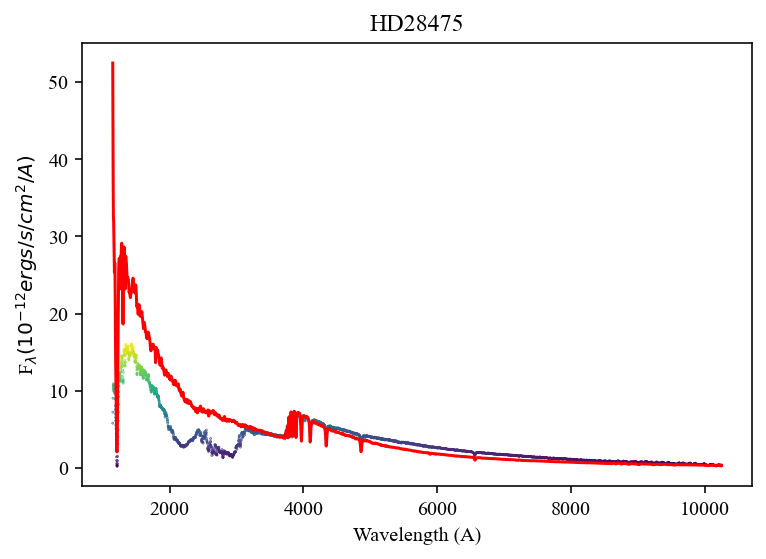
\includegraphics[scale = .5]{first.png}
        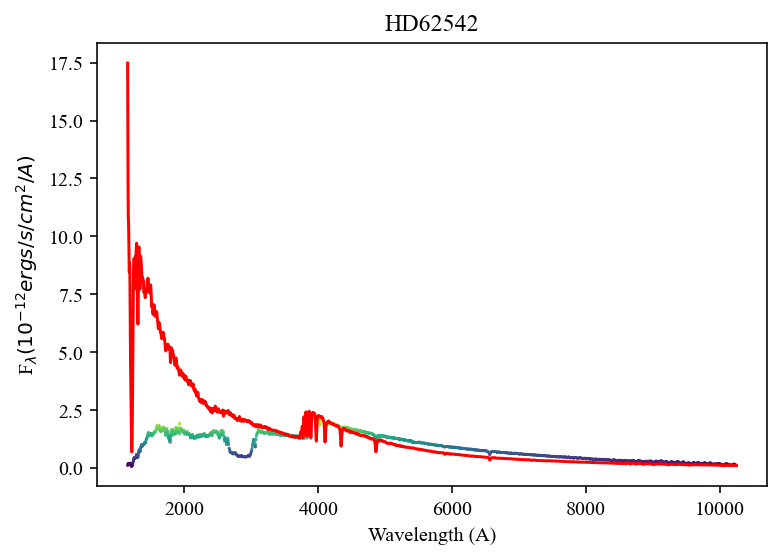
\includegraphics[scale = .5]{second.png}
    \end{figure}

    When producing the graphs, we simply scaled the template up or down to best fit the actual spectrum.
    However, We cannot use our scaling values for the flux ratios. We need to take the ratio of the \textit{scaled} template spectrum emission in the $V$ band to the actual stellar emission in the $V$ band.
    This way we get a correct $A_V$ value. The following code gives correct flux ratios, by taking the maximum values of the scaled and actual spectra and giving a ratio.

    \begin{python}
        # -*- coding: utf-8 -*-
        """
        Created on Wed Jan 29 15:05:27 2025

        @author: cmark
        """

        import pandas as pd
        import matplotlib.pyplot as plt
        import numpy as np
        import os

        os.chdir("C:/Users/cmark/Spyder/PHSCS 428/")

        HD1data = pd.read_table("HD28745.txt", delim_whitespace = 'true')

        HD2data = pd.read_table("HD62542.txt", delim_whitespace= 'true')

        BVdata = pd.read_table("B57V.txt", delim_whitespace= 'true')

        # setting fonts and stuff.
        plt.rcParams['font.family'] = 'Times New Roman'
       

        HD1_clean = HD1data[(HD1data['#Wavelength(Ang.A)'] >= 1200) & (HD1data['#Wavelength(Ang.A)'] <= 1800) ]
        HD2_clean = HD2data[(HD1data['#Wavelength(Ang.A)'] >= 1200) & (HD2data['#Wavelength(Ang.A)'] <= 1800) ]
        template_clean = BVdata[(BVdata['#Wavelength(Ang.A)'] >= 1200) & (BVdata['#Wavelength(Ang.A)'] <= 1800) ]

        HD1max_clean = HD1_clean['F_lambda(10^-12ergs/s/cm^2/A)'].max()
        HD2max_clean = HD2_clean['F_lambda(10^-12ergs/s/cm^2/A)'].max()
        BVmax_clean1 = 2.4* template_clean['F_lambda(10^-12ergs/s/cm^2/A)'].max()
        BVmax_clean2 = .8 * template_clean['F_lambda(10^-12ergs/s/cm^2/A)'].max()


        # printing 

        print(f'HD 28475 Max: {HD1max_clean}')
        print(f'HD 62542 Max: {HD2max_clean}')
        print(f'Template 1 Max (Scaled): {BVmax_clean1}')
        print(f'Template 2 Max (Scaled): {BVmax_clean2}')



        ratio_actual1 = HD1max_clean / BVmax_clean1
        ratio_actual2 = HD2max_clean / BVmax_clean2

        print(f'HD 28475 Actual Flux Ratio: {ratio_actual1}')
        print(f'HD 62542 Actual Flux Ratio: {ratio_actual2}')
    \end{python}

    The results:

    \begin{center}
        \begin{tabular}{|c | c | c | c|}
        \hline
        Star & Spectral Type & Flux Ratio & $A_V$ \\
        \hline
        HD 28475 & B5V C & .5516 & .645 \\
        HD 62542 & B3V C & .1991 & 1.752 \\
        \hline
        \end{tabular}
    \end{center}

    \subsection{}
    The graphs:

    \begin{figure}[H]
        \centering
        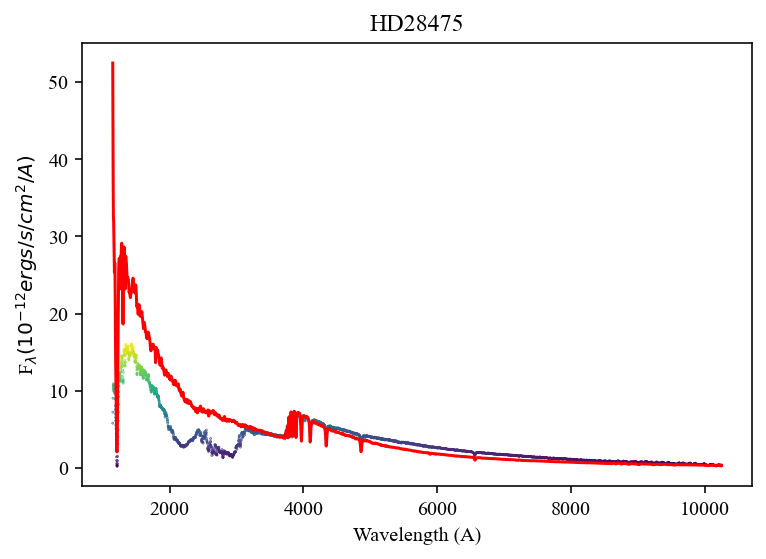
\includegraphics[scale = .5]{first.png}
        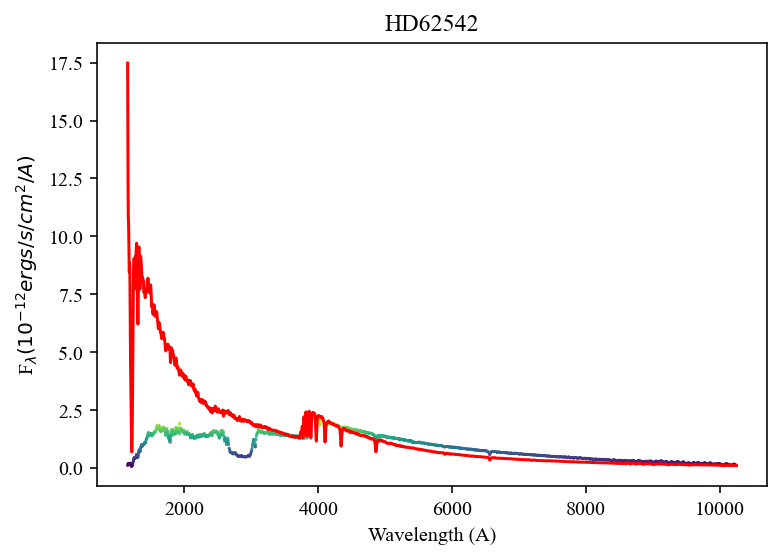
\includegraphics[scale = .5]{second.png}
    \end{figure}

    \subsection{}

    Here are the results.

    \begin{figure}[H]
        \centering
        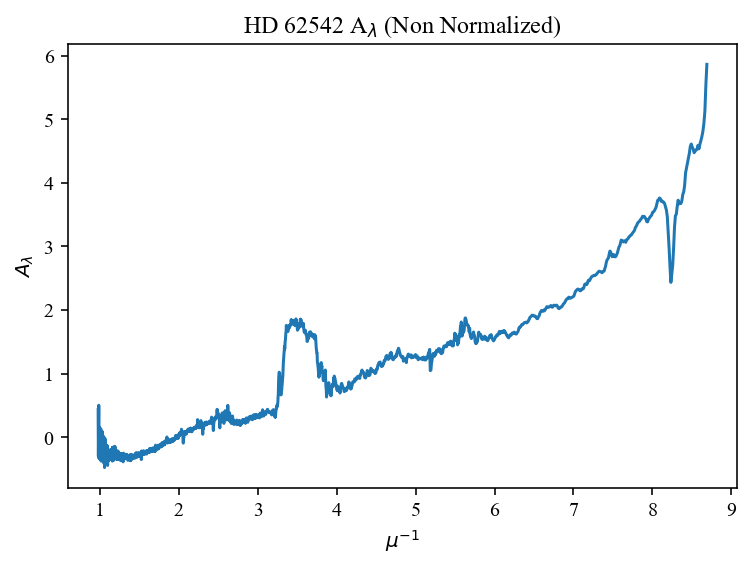
\includegraphics[scale = .5]{Figure 2025-02-02 013752 (0).png}
        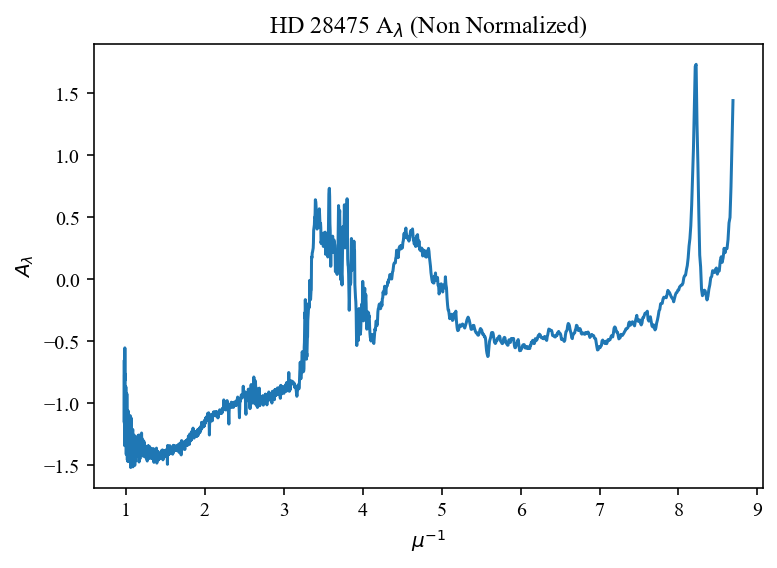
\includegraphics[scale = .5]{Figure 2025-02-02 013752 (1).png}
        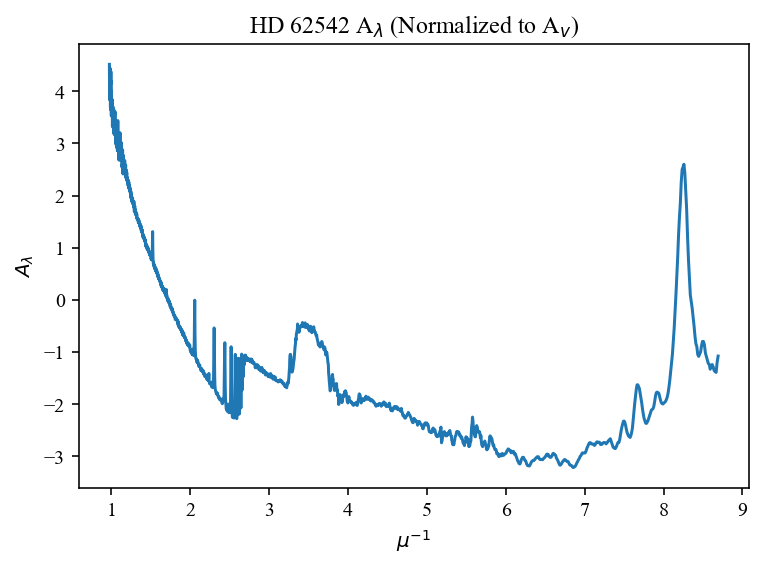
\includegraphics[scale = .5]{Figure 2025-02-02 013752 (2).png}
        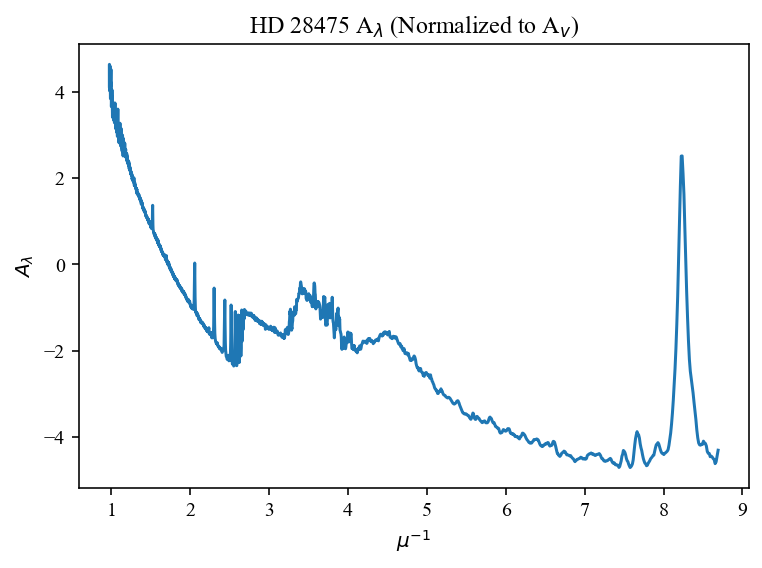
\includegraphics[scale = .5]{Figure 2025-02-02 013752 (3).png}
    \end{figure}

    And the code:

    \begin{python}
        # ...
        #%%
        HD1conv = HD1data.copy()
        HD1conv['#Wavelength(Ang.A)'] = HD1conv['#Wavelength(Ang.A)'] * 1e-4
        x = 1 / HD1conv['#Wavelength(Ang.A)']

        Alambda1 = -2.5 * np.log10(HD1data['F_lambda(10^-12ergs/s/cm^2/A)'] / 2.4*BVdata['F_lambda(10^-12ergs/s/cm^2/A)'])

        plt.figure()
        plt.title('HD 28475 A$_{\lambda}$ (Normalized to A$_v$)')
        plt.xlabel('$\mu^{-1}$')
        plt.ylabel("$A_\lambda$")
        plt.plot(x, Alambda1)

        #%%
        HD2conv = HD2data.copy()
        HD2conv['#Wavelength(Ang.A)'] = HD2conv['#Wavelength(Ang.A)'] * 1e-4
        x = 1 / HD2conv['#Wavelength(Ang.A)']

        Alambda2 = -2.5 * np.log10(HD2data['F_lambda(10^-12ergs/s/cm^2/A)'] / .8*BVdata['F_lambda(10^-12ergs/s/cm^2/A)'])

        plt.figure()
        plt.title('HD 62542 A$_{\lambda}$ (Normalized to A$_v$)')
        plt.xlabel('$\mu^{-1}$')
        plt.ylabel("$A_\lambda$")
        plt.plot(x, Alambda2)
    \end{python}

    \subsection{}

    Knowing that $R_V = \tfrac{A_V}{E(B - V)}$, we can read $R_V$ from the slope. We exclude the ranges $\approx 120 nm \approx 8.3$ and $241 nm \approx 3.5$.
    We obtained slopes of:

    \begin{center}
    \begin{tabular}{| c | c | c |}
        \hline
        Star & RV 1 & RV 2 \\
        \hline
        HD 28475 & 0.3816 & 0.02365\\
        HD 62542 & 0.4444 & 0.5638 \\
        \hline
    \end{tabular}
    \end{center}

    \begin{figure}[H]
        \centering
        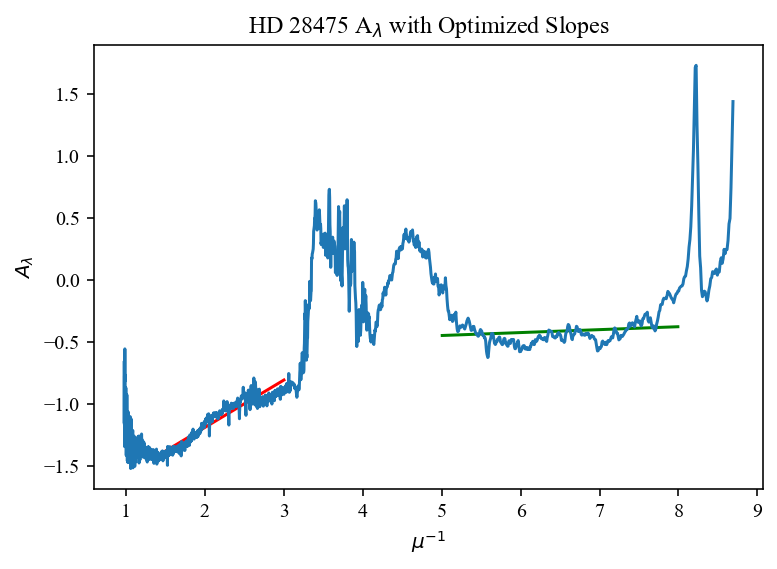
\includegraphics[scale = .5]{sl1.png}
        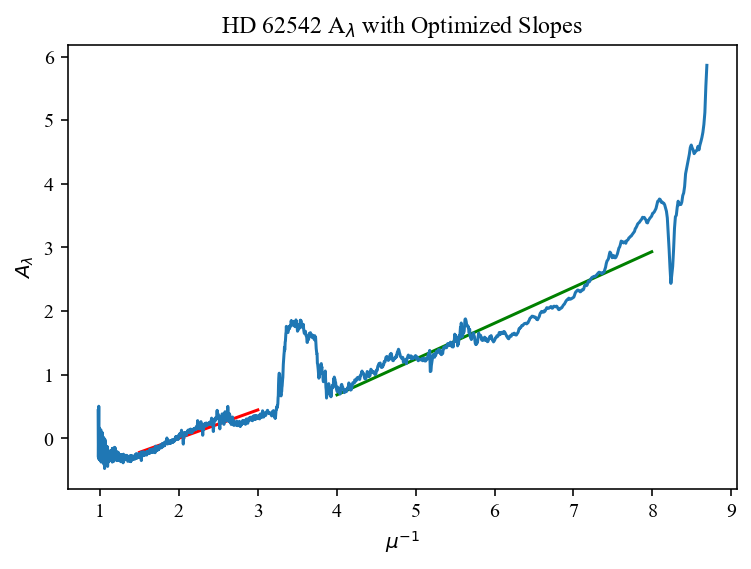
\includegraphics[scale = .5]{sl2.png}
    \end{figure}

    \subsection{}
    The increase in $A_\lambda$ at about 4.5 may be due to a number of factors.
    It corresponds to a wavelength of about 200 nanometers.

    \begin{enumerate}
        \item Dust grain size along our line of sight to HD 28475 may be of similar size to that wavelength.
        \item There may be more dust along our line of sight. 
        \item Dust or molecular compound properties may be of the optimal absorbing size.
    \end{enumerate}

    \subsection{}
    Differences between the curves may be due to generl abnormalities in the dust.
    We also are only accounting for one kind of extinction, which may not be entirely accurate.
    Another instance of discrepancy may be due to our use of templataes. I only scaled until it seemed visually correct.
    I also just used a standard value for color excess that may not be entirely accurate for the stars. 
    The slopes I calculated are also linear approximations and therefore not as accurate as we would hope.
\end{document}